\documentclass[twoside]{book}

% Packages required by doxygen
\usepackage{fixltx2e}
\usepackage{calc}
\usepackage{doxygen}
\usepackage[export]{adjustbox} % also loads graphicx
\usepackage{graphicx}
\usepackage[utf8]{inputenc}
\usepackage{makeidx}
\usepackage{multicol}
\usepackage{multirow}
\PassOptionsToPackage{warn}{textcomp}
\usepackage{textcomp}
\usepackage[nointegrals]{wasysym}
\usepackage[table]{xcolor}

% Font selection
\usepackage[T1]{fontenc}
\usepackage[scaled=.90]{helvet}
\usepackage{courier}
\usepackage{amssymb}
\usepackage{sectsty}
\renewcommand{\familydefault}{\sfdefault}
\allsectionsfont{%
  \fontseries{bc}\selectfont%
  \color{darkgray}%
}
\renewcommand{\DoxyLabelFont}{%
  \fontseries{bc}\selectfont%
  \color{darkgray}%
}
\newcommand{\+}{\discretionary{\mbox{\scriptsize$\hookleftarrow$}}{}{}}

% Page & text layout
\usepackage{geometry}
\geometry{%
  a4paper,%
  top=2.5cm,%
  bottom=2.5cm,%
  left=2.5cm,%
  right=2.5cm%
}
\tolerance=750
\hfuzz=15pt
\hbadness=750
\setlength{\emergencystretch}{15pt}
\setlength{\parindent}{0cm}
\setlength{\parskip}{3ex plus 2ex minus 2ex}
\makeatletter
\renewcommand{\paragraph}{%
  \@startsection{paragraph}{4}{0ex}{-1.0ex}{1.0ex}{%
    \normalfont\normalsize\bfseries\SS@parafont%
  }%
}
\renewcommand{\subparagraph}{%
  \@startsection{subparagraph}{5}{0ex}{-1.0ex}{1.0ex}{%
    \normalfont\normalsize\bfseries\SS@subparafont%
  }%
}
\makeatother

% Headers & footers
\usepackage{fancyhdr}
\pagestyle{fancyplain}
\fancyhead[LE]{\fancyplain{}{\bfseries\thepage}}
\fancyhead[CE]{\fancyplain{}{}}
\fancyhead[RE]{\fancyplain{}{\bfseries\leftmark}}
\fancyhead[LO]{\fancyplain{}{\bfseries\rightmark}}
\fancyhead[CO]{\fancyplain{}{}}
\fancyhead[RO]{\fancyplain{}{\bfseries\thepage}}
\fancyfoot[LE]{\fancyplain{}{}}
\fancyfoot[CE]{\fancyplain{}{}}
\fancyfoot[RE]{\fancyplain{}{\bfseries\scriptsize Generated by Doxygen }}
\fancyfoot[LO]{\fancyplain{}{\bfseries\scriptsize Generated by Doxygen }}
\fancyfoot[CO]{\fancyplain{}{}}
\fancyfoot[RO]{\fancyplain{}{}}
\renewcommand{\footrulewidth}{0.4pt}
\renewcommand{\chaptermark}[1]{%
  \markboth{#1}{}%
}
\renewcommand{\sectionmark}[1]{%
  \markright{\thesection\ #1}%
}

% Indices & bibliography
\usepackage{natbib}
\usepackage[titles]{tocloft}
\setcounter{tocdepth}{3}
\setcounter{secnumdepth}{5}
\makeindex

% Hyperlinks (required, but should be loaded last)
\usepackage{ifpdf}
\ifpdf
  \usepackage[pdftex,pagebackref=true]{hyperref}
\else
  \usepackage[ps2pdf,pagebackref=true]{hyperref}
\fi
\hypersetup{%
  colorlinks=true,%
  linkcolor=blue,%
  citecolor=blue,%
  unicode%
}

% Custom commands
\newcommand{\clearemptydoublepage}{%
  \newpage{\pagestyle{empty}\cleardoublepage}%
}

\usepackage{caption}
\captionsetup{labelsep=space,justification=centering,font={bf},singlelinecheck=off,skip=4pt,position=top}

%===== C O N T E N T S =====

\begin{document}

% Titlepage & ToC
\hypersetup{pageanchor=false,
             bookmarksnumbered=true,
             pdfencoding=unicode
            }
\pagenumbering{roman}
\begin{titlepage}
\vspace*{7cm}
\begin{center}%
{\Large My Project }\\
\vspace*{1cm}
{\large Generated by Doxygen 1.8.11}\\
\end{center}
\end{titlepage}
\clearemptydoublepage
\tableofcontents
\clearemptydoublepage
\pagenumbering{arabic}
\hypersetup{pageanchor=true}

%--- Begin generated contents ---
\chapter{Namespace Index}
\section{Namespace List}
Here is a list of all documented namespaces with brief descriptions\+:\begin{DoxyCompactList}
\item\contentsline{section}{\hyperlink{namespacesuma}{suma} \\*Script para sumar }{\pageref{namespacesuma}}{}
\end{DoxyCompactList}

\chapter{File Index}
\section{File List}
Here is a list of all documented files with brief descriptions\+:\begin{DoxyCompactList}
\item\contentsline{section}{\hyperlink{ARN_8cpp}{A\+R\+N.\+cpp} }{\pageref{ARN_8cpp}}{}
\item\contentsline{section}{{\bfseries A\+R\+N.\+h} }{\pageref{ARN_8h}}{}
\end{DoxyCompactList}

\chapter{Namespace Documentation}
\hypertarget{namespacesuma}{}\section{suma Namespace Reference}
\label{namespacesuma}\index{suma@{suma}}


Script para sumar.  


\subsection*{Functions}
\begin{DoxyCompactItemize}
\item 
def \hyperlink{namespacesuma_a9d2207a78036e4a01305926f9af97137}{sumar} (data)
\begin{DoxyCompactList}\small\item\em Esta función suma los elementos de una lista. \end{DoxyCompactList}\end{DoxyCompactItemize}
\subsection*{Variables}
\begin{DoxyCompactItemize}
\item 
list {\bfseries datos} = \mbox{[}$\,$\mbox{]};\hypertarget{namespacesuma_aa8d49a7f299460afb239339e04409261}{}\label{namespacesuma_aa8d49a7f299460afb239339e04409261}

\end{DoxyCompactItemize}


\subsection{Detailed Description}
Script para sumar. 

\subsection{Function Documentation}
\index{suma@{suma}!sumar@{sumar}}
\index{sumar@{sumar}!suma@{suma}}
\subsubsection[{\texorpdfstring{sumar(data)}{sumar(data)}}]{\setlength{\rightskip}{0pt plus 5cm}def suma.\+sumar (
\begin{DoxyParamCaption}
\item[{}]{data}
\end{DoxyParamCaption}
)}\hypertarget{namespacesuma_a9d2207a78036e4a01305926f9af97137}{}\label{namespacesuma_a9d2207a78036e4a01305926f9af97137}


Esta función suma los elementos de una lista. 


\begin{DoxyParams}{Parameters}
{\em data} & la lista. \\
\hline
\end{DoxyParams}
\begin{DoxyReturn}{Returns}
el resultado de la suma. 
\end{DoxyReturn}

\chapter{File Documentation}
\hypertarget{suma_8c}{}\section{suma.\+c File Reference}
\label{suma_8c}\index{suma.\+c@{suma.\+c}}
{\ttfamily \#include $<$stdio.\+h$>$}\\*
{\ttfamily \#include $<$stdlib.\+h$>$}\\*
Include dependency graph for suma.\+c\+:\nopagebreak
\begin{figure}[H]
\begin{center}
\leavevmode
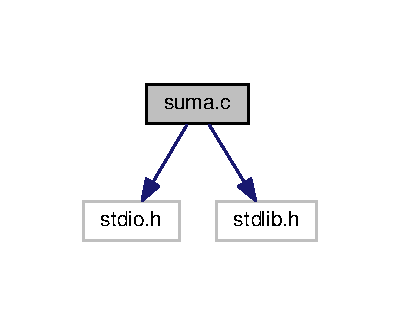
\includegraphics[width=192pt]{suma_8c__incl}
\end{center}
\end{figure}
\subsection*{Functions}
\begin{DoxyCompactItemize}
\item 
double \hyperlink{suma_8c_aa827d9b7c26ade2f875045704d50ff6c}{sumar} (int size, double $\ast$array)
\item 
int {\bfseries main} (int argc, char $\ast$$\ast$argv)\hypertarget{suma_8c_a3c04138a5bfe5d72780bb7e82a18e627}{}\label{suma_8c_a3c04138a5bfe5d72780bb7e82a18e627}

\end{DoxyCompactItemize}


\subsection{Detailed Description}
Programa que suma 

\subsection{Function Documentation}
\index{suma.\+c@{suma.\+c}!sumar@{sumar}}
\index{sumar@{sumar}!suma.\+c@{suma.\+c}}
\subsubsection[{\texorpdfstring{sumar(int size, double $\ast$array)}{sumar(int size, double *array)}}]{\setlength{\rightskip}{0pt plus 5cm}double sumar (
\begin{DoxyParamCaption}
\item[{int}]{size, }
\item[{double $\ast$}]{array}
\end{DoxyParamCaption}
)}\hypertarget{suma_8c_aa827d9b7c26ade2f875045704d50ff6c}{}\label{suma_8c_aa827d9b7c26ade2f875045704d50ff6c}
Esta función toma un arreglo de números reales y devuelve la suma de todos sus elementos. 
\begin{DoxyParams}{Parameters}
{\em size} & tamaño del arreglo. \\
\hline
{\em array} & arreglo de numeros reales. \\
\hline
\end{DoxyParams}
\begin{DoxyReturn}{Returns}
resultado de la suma. 
\end{DoxyReturn}

\hypertarget{suma_8cpp}{}\section{suma.\+cpp File Reference}
\label{suma_8cpp}\index{suma.\+cpp@{suma.\+cpp}}
{\ttfamily \#include $<$iostream$>$}\\*
{\ttfamily \#include $<$vector$>$}\\*
{\ttfamily \#include $<$string$>$}\\*
Include dependency graph for suma.\+cpp\+:\nopagebreak
\begin{figure}[H]
\begin{center}
\leavevmode
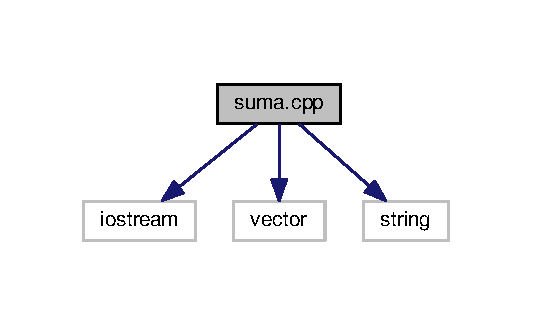
\includegraphics[width=256pt]{suma_8cpp__incl}
\end{center}
\end{figure}
\subsection*{Functions}
\begin{DoxyCompactItemize}
\item 
double \hyperlink{suma_8cpp_ace45d376a739eb1851a7bf8d0a73ed47}{sumar} (vector$<$ double $>$)
\item 
int {\bfseries main} (int argc, char $\ast$argv\mbox{[}$\,$\mbox{]})\hypertarget{suma_8cpp_a0ddf1224851353fc92bfbff6f499fa97}{}\label{suma_8cpp_a0ddf1224851353fc92bfbff6f499fa97}

\end{DoxyCompactItemize}


\subsection{Detailed Description}
Programa que suma 

\subsection{Function Documentation}
\index{suma.\+cpp@{suma.\+cpp}!sumar@{sumar}}
\index{sumar@{sumar}!suma.\+cpp@{suma.\+cpp}}
\subsubsection[{\texorpdfstring{sumar(vector$<$ double $>$)}{sumar(vector< double >)}}]{\setlength{\rightskip}{0pt plus 5cm}double sumar (
\begin{DoxyParamCaption}
\item[{vector$<$ double $>$}]{args}
\end{DoxyParamCaption}
)}\hypertarget{suma_8cpp_ace45d376a739eb1851a7bf8d0a73ed47}{}\label{suma_8cpp_ace45d376a739eb1851a7bf8d0a73ed47}
Esta función toma un vector de números reales y devuelve la suma de todos sus elementos. 
\begin{DoxyParams}{Parameters}
{\em args} & std\+::vector$<$double$>$ que contiene los argumentos. \\
\hline
\end{DoxyParams}
\begin{DoxyReturn}{Returns}
resultado de la suma. 
\end{DoxyReturn}

%--- End generated contents ---

% Index
\backmatter
\newpage
\phantomsection
\clearemptydoublepage
\addcontentsline{toc}{chapter}{Index}
\printindex

\end{document}
